\chapter{Montage de l’écran LCD}

\section{Présentation écran}
\begin{figure}[h]
	\centering
	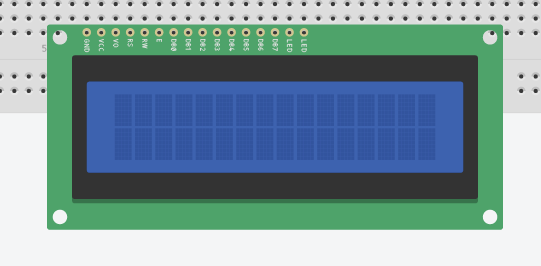
\includegraphics[width=0.5\linewidth]{lcd.png}
    \caption{Écran LCD}
    \label{lcd}
\end{figure}
Au cours de ce projet nous allons utiliser un écran LCD 16x2 équipé du driver Hitachi HD44780 (figure \ref{lcd}). Ce type d'écran est compatible avec la librairie \og LiquidCrystal \fg disponible nativement au sein de l'IDE\footnotemark Arduino 

%%
 \footnotetext[1]{IDE: Entegrated Eevelopment Environment ; ou EDI en français: Environnement de Développement Intégré.
 	source \href{https://en.wikipedia.org/wiki/Integrated_development_environment}{Wikipedia}}
%%

\begin{figure}[h]
	\centering
	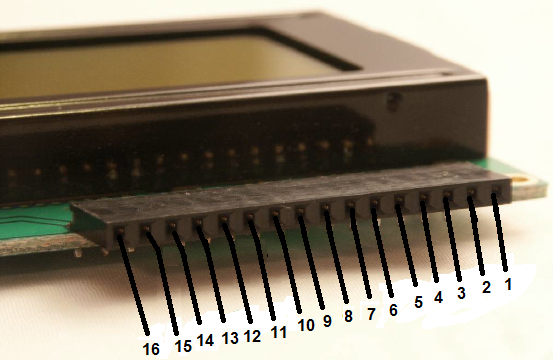
\includegraphics[width=12cm]{HD44780-LCD-pinout.png}
    \caption{Pin écran LCD}
    \label{PinLCD}    
\end{figure}


\paragraph{}
	Description des pins :
    \begin{enumerate}[label=\arabic*]
    	\item Vss - Masse 0V de l'écran LCD.
		\item Vcc - Pin d'alimentation de l'écran. Le voltage accepté est entre 3.3V et 5V.
		\item Pin d'ajustement du contraste. On y branche un potentiomètre pour faire varier le contraste.
		\item Pin sélection du registre. Si égale a 0 : mode commande, si égale a 1 : mode données.
		\item Pin de lecture/écriture. Si égale a 0 : mode écriture, si égale a 1 : mode lecture.
		\item Pin de validation.
		\item Bus de données, bit 0
		\item Bus de données, bit 1
		\item Bus de données, bit 2
		\item Bus de données, bit 3
		\item Bus de données, bit 4
		\item Bus de données, bit 5
		\item Bus de données, bit 6
		\item Bus de données, bit 7
		\item Alimentation du rétroéclairage de l'écran. La tension d'entré maximale est 5V et correspond a l'éclairage maximum. On peut y connecter un potentiomètre pour faire varier l'intensité du rétroéclairage.
		\item Pin de terre du rétroéclairage.
    \end{enumerate}
    
\newpage
\section{Montage}
\begin{figure}[h]
	\centering
	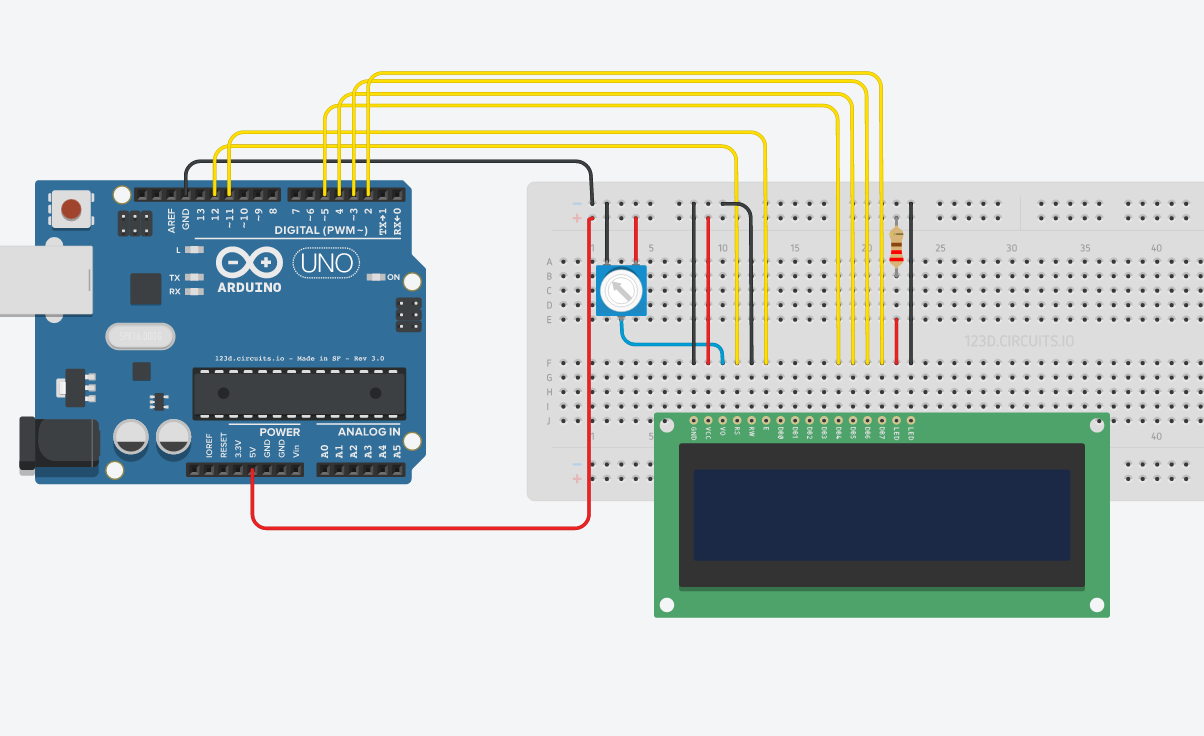
\includegraphics[width=\linewidth]{montageLCD.png}
    \caption{Montage écran LCD}
    \label{montageLCD}    
\end{figure}
Pour le montage de l'écran LCD et de l'Arduino (figure \ref{montageLCD}) nous avons utilisés :
\begin{itemize}
	\item 1 écran LCD,
    \item 1 potentiomètre $10k\Omega$,
    \item 1 Arduino Uno,
    \item 1 résistance $220\Omega$,
    \item 5 fil noir,
    \item 4 fil rouge,
    \item 1 fil bleu,
    \item 6 fil jaune.
\end{itemize}

